\section{Evaluation}
\label{sec:eval}

In this section, we evaluate \ouralgo's algorithm on a large set of path
changes. Our evaluation goals are to demonstrate that our approach is 1)
\emph{accurate} in terms of always including the root cause in the
suspect set; 2) \emph{precise} in that it identifies a small suspect set
(ideally of size one); 3) \emph{robust} to missing measurement from
vantage points; and 4) \emph{scalable} in that it does not require
monitoring a prohibitive number of paths and it can identify root causes
within minutes of paths changing. To evaluate these goals, we use
controlled path changes on real Internet paths, simulations for larger
topologies, and path changes ``in the wild.'' In contrast to previous
work, our approach is both precise and accurate, largely because it
accounts for induced path changes. Further, we show that our results are
similar even with only partial information from paths in the monitoring
set for a prefix.

%the accuracy of our algorithm on path changes
%obtained via controlled announcements
%to the Internet, an empirically informed simulation and path changes observed in the wild.
%With the help of controlled announcements from our TP testbed, we cause link
%failures and restorations at strategic locations to cause BGP path changes. 
%For all such path changes, our algorithm is able to put the root cause AS in its
%final suspect set and prunes the suspect set to contain just the root cause AS more than 75\%
%of the time.
%To show the full efficacy of our approach we simulate induced path changes in an empirically
%informed Internet topology and show that our root cause analysis 
%algorithm isolates the failure in most cases.  Our algorithm performs very well on 
%these in-the-wild path changes as well. Overall we show that that our system, deployed in
%real-time, identifies the root cause of BGP path changes with high accuracy,
%with a fairly light measurement footprint.

\subsection{Controlled Internet Experiments}

In this section, we use controlled experiments on real Internet paths to demonstrate the accuracy and  
precision of \ouralgo for identifying the root cause of a path change. We begin 
by describing our experiment methodology, then present a case study of how our algorithm works on a real 
induced path change. Last, we use a large set of AS-link failures to
evaluate our approach and compare it with \feldmann~\cite{feldman}.

\subsubsection{Methodology}

A key challenge for evaluating root cause analysis algorithms is the
lack of control or ground truth for interdomain path changes.  Our work
addresses this using the Transit Portal (TP) platform~\cite{bgpmux} to
craft announcements that cause controllable path changes for real
Internet paths. Specifically, we use BGP poisoning~\cite{optometry} to
induce changes for paths toward a prefix we control.\footnote{We use the
same conservative approach to poisoning as described in
\S\ref{subsec:candidates}.} Because such announcements cause the
targeted AS to withdraw routes from its upstream neighbors, we know that
the ``root cause'' for the corresponding path change is the targeted AS.
Likewise, when unpoisoning a prefix, we effectively emulate a ``link
up'' event for the targeted AS.

We use five /24 \emph{poisoning} prefixes to cause path changes.  
Each prefix is announced from one of the five TP sites:
University of Washington, University of Wisconsin, Georgia Tech,
Princeton University, and Clemson University.
We perform a sequence of poisonings using the same
topology discovery scheme described in \S\ref{subsec:candidates},
starting the discovery process from the ASes where we have a PlanetLab
vantage point.  We change announcements (add or remove poisonings) at
most once every 90 minutes to allow for BGP convergence and to avoid
flap dampening effects. 
In addition to changes caused by our poisoned announcements, paths may 
change in response to exogenous events. To account for this, we announce 
a separate \emph{sentinel} /24 prefix from each TP site and do not vary its AS-Path. If 
the sentinel and poisoning prefixes change at the same time, then it is likely 
caused by an exogenous event and we filter the change from our dataset.

We let the experiment run for one week starting November 25th, 2012,
yielding a total of 105 distinct poisonings for each prefix.  The
BGP updates and traceroutes collected throughout the experiment traverse
351 ASes and include 2572 path changes. Many of these path changes
are duplicates, and are therefore ignored. 
%We also ignore all
%experiments where the path remains stable even though it traverses the
%poisoned AS (\ie the poisoned announcement did not trigger BGP loop
%prevention). 
Similarly, we also ignore experiments where we detect that
one of the poisoned AS's peers filtered the poisoned announcement.
After applying the filters, our experiments yield 638 unique
path changes.  

\begin{comment}
To obtain AS paths to our prefixes, we collect paths from:
1) BGP route collectors \cite{ripe-ris, routeviews}, 2) traceroutes from
approximately 200 PlanetLab nodes to the collected every 10 minutes, and
3) reverse paths from a set of iPlane PoPs \cite{iplane-web} using
Reverse Traceroute \cite{revtr}. We use IP-to-AS mapping provided by
\emph{iPlane} to get AS level paths from traceroutes.
\end{comment}

\begin{comment} % {{{
We employ a modified version of Breadth-First Search on the paths
collected from these vantage points to explore new paths: whenever a
poisoning results in a new path, the newly discovered ASes are poisoned
in turn until all paths were exhausted.  An example is shown in \fig~\ref{fig:bfs}. Starting with the next-hop of the vantage point $V$, a
poison stack is created such that the AS closest to the destination,
i.e., $B$ is the first to get poisoned. Poisoning $B$ reveals a path
through $C$ that $A$ can take to $D$. But poisoning $B$ and $C$ together
disconnects $A$ from $D$. This leads us to believe that $A$ has two
working paths toward $D$: one through $B$ and the other through $C$, and
that the path through $B$ is preferred over the path through $C$. The
next poisoning in the stack is $A$, which will be issued after the
withdrawing the earlier poisonings so that the path returns to its
natural state. 

\begin{figure}[!htbp]
\centering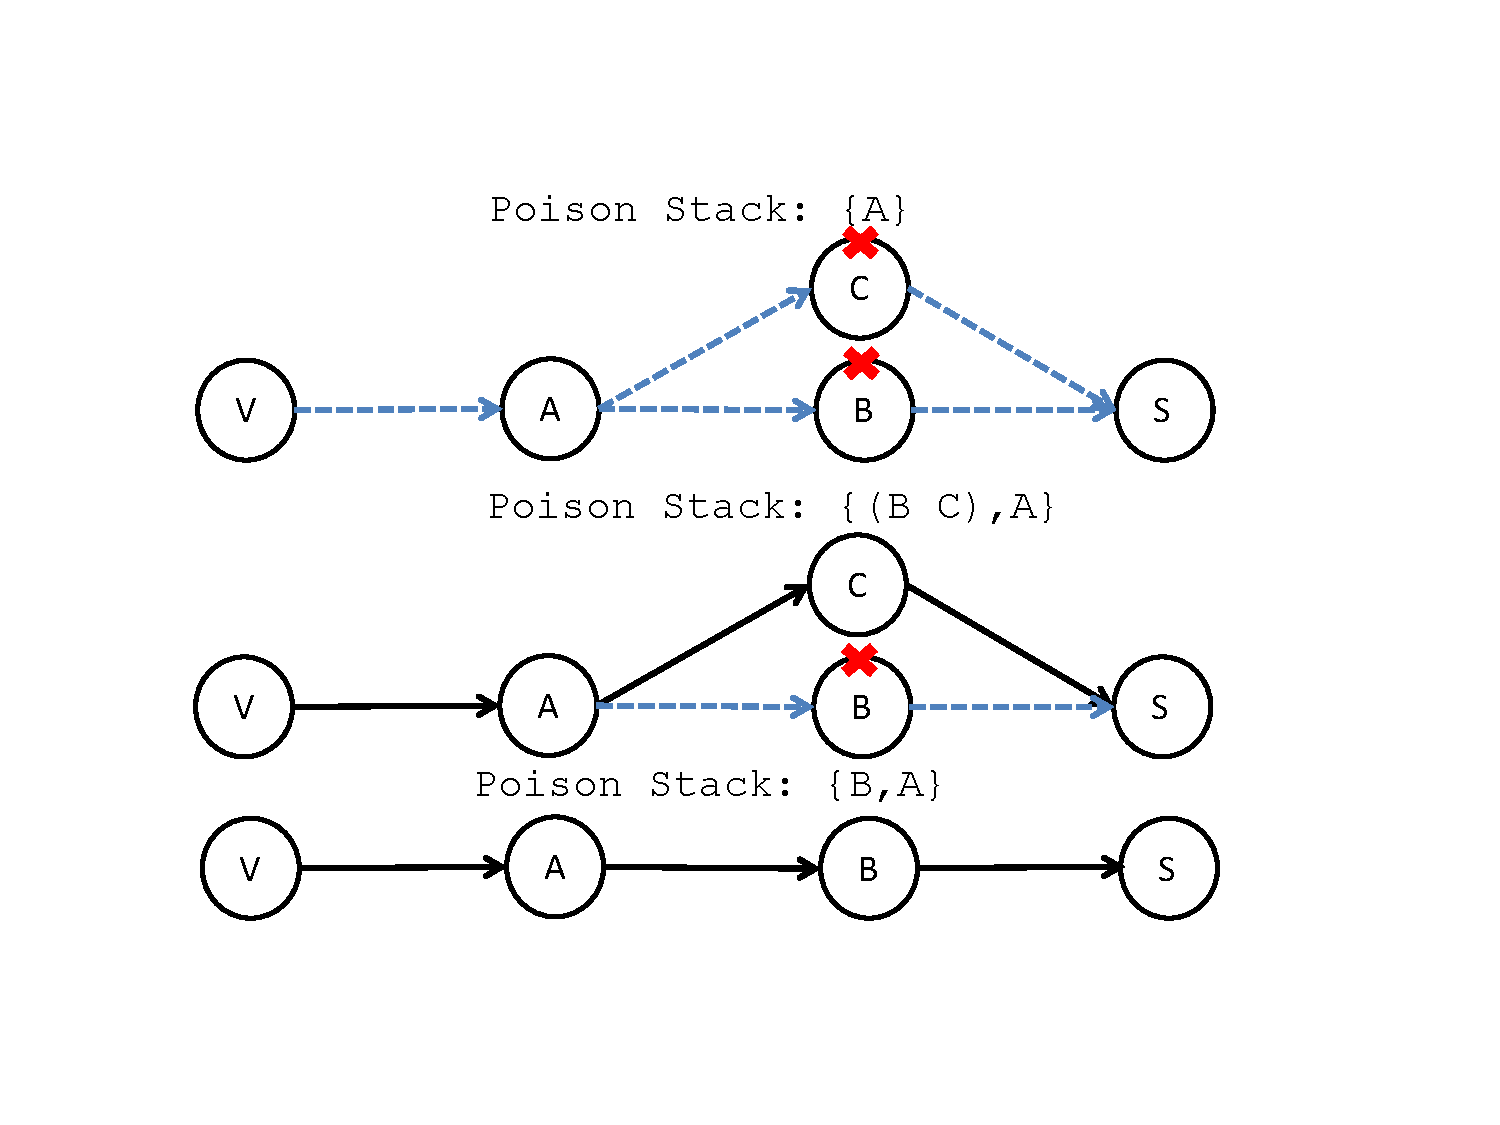
\includegraphics[width=\columnwidth]{figs/bfs.pdf} \caption{A
Breadth-First Search like algorithm for discovering all possible AS-level paths
between vantage point $V$ and destination $D$. After poisoning $B$ and $C$
together, $V$ gets disconnected from $D$, leaving only $A$ in the poison stack.}
\label{fig:bfs} 
\end{figure}
\end{comment} % }}}


\subsubsection{Induced Path Change Case Study}

We begin by describing how \ouralgo locates the root cause AS for an induced path
change via a case study. Note that since the root cause AS lies neither on the old nor the 
new path,  \feldmann will not be able to find it. The path change takes place between the National Taiwan University
(NTU, ASN: 17716) and our experimental AS (ASN: 47065). We used TP to announce prefix
184.164.249.0/24 from the University of Wisconsin (ASN: 2381)
and poisoned TRANSPAC (ASN: 22388) at 2:22 AM PST on November 27th, 2012. After convergence a path change was observed at a PlanetLab node located in 
NTU at 2:35 AM. The AS-level path change is shown in \fig~\ref{fig:case-study}.

\begin{figure}[tb]
\centering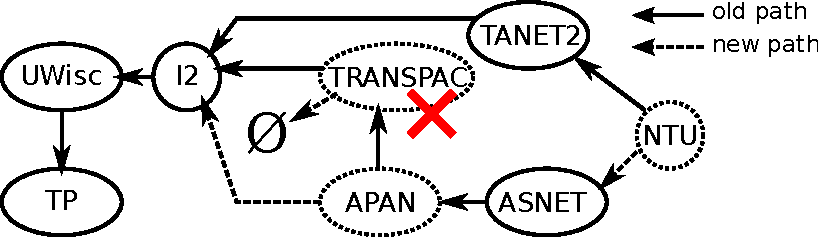
\includegraphics[width=\columnwidth]{figs/case-study.pdf}
\vspace{-1.2em}
\caption{Case study for an induced path change. The path change is caused by
a poisoned announcement that emulates a link failure at TRANSPAC (AS: 22388).}
\label{fig:case-study}
\vspace{.7em}
\end{figure}

%Initially NTU was using the path through TANET2-TW (ASN: 7539) which passed
%through Internet2 to reach UWisc. Our historical path database, as well as the path 
%to the sentinel prefix, shows that this 
%is the default AS path used by NTU for UWisc. Poisoning TRANSPAC (ASN: 22388) causes TRANSPAC to withdraw its path through Internet2 (ASN: 11537) from APAN-JP (ASN: 7660). This forces APAN-JP to switch to its next-best path that 
%uses a direct peering with Internet2. NTU receives this new path from the 
%Academic Sinica Network (ASNET, ASN: 9264) and starts using it instead of its
%default path through TANET2-TW. This is the path change observed
%at the PlanetlLab vantage point inside NTU. 
%
%Upon observing the path change at NTU, our root cause algorithm probes the path from TANET2
%after the poisoning and finds that it was the same path before the poisoning, i.e., TANET2 $\rightarrow$ 
%Internet2 $\rightarrow$ UWisc $\rightarrow$ GENI. This eliminates TANET2 as well as Internet2,
%UWisc and GENI from the suspect set. It then probes ASNET's old path and discovers that it
%contained a previously undiscovered AS, i.e., TRANSPAC. TRANSPAC is then added to the suspect set.
%Since we assume single failures, at this stage NTU is ruled out as the root cause because one of its successors, i.e., ASNET had different before and after paths. Now TRANSPAC is queried
%for its path after the poisoning and we discover that it withdrew its
%announcement, thus eliminating its predecessors APAN-JP and ASNET from the suspect set. Since there are no more ASes left to probe, we conclude that TRANSPAC is the root cause. 
%In addition to the knowledge that we poisoned TRANSPAC, we have also
%checked with TRANSPAC's NOC that it would withdraw its announcement for
%the prefix in such a case. 

Upon observing the path change at
NTU, \ouralgo runs \algstr~\ref{algo:practical} to identify the root
cause. It begins by adding ASes in NTU's old and new paths to the suspect
set. Then, it searches for the root cause in order of distance from NTU.
It first checks that TANET2 uses the same
path before and after the change, so TANET2 and all its downstream ASes 
cannot be the root cause of the change (\localC, lines 5--7).
We illustrate the algorithm in \tab~\ref{tab:case-study}, where each row shows the AS being currently visited
and the suspect set from the previous step.  For lack of space, we
do not show the TP AS and UWisc, which are trivially eliminated as root causes.
When \ouralgo visits ASNET, it
(i) removes NTU from the suspect set because ASNET changed paths (line~9),
and (ii) adds TRANSPAC from ASNET's old path
to the suspect set (line~13).
Similarly when it visits APAN, it removes ASNET from the suspect set since
APAN experienced a path change.
Finally, the algorithm visits TRANSPAC and removes APAN from the
suspect set (because TRANSPAC changed paths) and terminates returning
a suspect set containing only TRANSPAC, the correct root cause.
To validate our approach for obtaining ground truth via poisoning, we confirmed 
with TRANSPAC's NOC that it withdrew its announcement for our prefix.

\begin{table}
\begin{tabular}{ccl}
\textbf{Step} & \textbf{Visit} & \textbf{Suspect Set} \\
\hline
1 & TANET2 & NTU, TANET2, I2, ASNET, APAN \\
2 & ASNET & NTU, ASNET, APAN\\
3 & APAN & APAN, TRANSPAC, ASNET \\
4 & TRANSPAC & TRANSPAC, APAN \\
5 & $\emptyset$ & TRANSPAC
\end{tabular}
\vspace{-3mm}
\caption{Illustration of the suspect set when recursing through 
\algstr~\ref{algo:practical} for the induced path change
shown in \fig~\ref{fig:case-study}.}
\label{tab:case-study}
\vspace{.7em}
\end{table}

\begin{table*}[!htbp] \centering
%\ra{1.3}
\begin{tabular}{@{}lcccccccc@{}} \toprule
& \multicolumn{3}{c}{\textbf{accuracy of suspect set}} & &
\multicolumn{4}{c}{\textbf{suspect set size when accurate}}  \\  
\cmidrule{2-4} \cmidrule{6-9}
& \textbf{ground truth in set} & \textbf{empty} & \textbf{inaccurate} & & \textbf{mean} & \textbf{median} & \textbf{25th perc.} & \textbf{75th perc.} \\ \midrule
\textbf{\ouralgo} & 100.0\% & 0.0\% & 0.0\% & & 1.66 & 1 & 1 & 2 \\  
\textbf{\ouralgo-correlation across VPs} & 100.0\% & 0.0\% & 0.0\% & & 1.32 & 1 & 1 & 1  \\ 
\textbf{ \feldmann-standard} & 61.7\% & 38.3\% & 0.0\% & & 1.20 & 1 & 1 & 1 \\  
\textbf{ \feldmann-individualPath} & 91.1\% & 0.0\% & 8.9\% & & 2.70 & 2 & 1 & 3  \\  
\bottomrule
\end{tabular} 
\caption{Comparison of \ouralgo with \feldmann, the approach used in previous work~\cite{feldman}. \ouralgo is both accurate and precise: it never misses the root cause and nearly always produces a suspect set size of two or smaller. \feldmann trades off precision for accuracy in the face of induced path changes: \feldmann-standard misses the root cause in many cases but has small suspect set sizes; \feldmann-individualPath misses fewer root causes but exhibits larger suspect set sizes.} 
\label{tab:feldmann} 
\end{table*}



\subsubsection{Controlled Internet Experiments}  
\label{sec:poisonings}

In this section, we use controlled experiments to show that \ouralgo is
accurate (always includes the root cause), precise (identifies suspect
sets of size 2 or smaller 96\% of the time) and robust to missing path
information (more than 50\% of paths must be missing to significantly
impact suspect set size). By comparison, previous work cannot be both
accurate and precise in the face of induced path changes, which occur
frequently. Further, we show that our approach is scalable in that it
monitors only a reasonable number
of paths and provides results within minutes of path changes. 

%We evaluate the accuracy our algorithm on path changes obtained through
%BGP poisonings with two objectives in mind: (1) the final candidate set
%should contain the ground truth (AS poisoned or unpoisoned), and (2) the
%final suspect set should be as small as possible, ideally containing
%only the poisoned or unpoisoned AS.  Our evaluation shows that the
%suspect set contained the poisoned AS for all path changes in the
%experiment, confirming that the algorithm is highly accurate.  Further,
%we find that the standard version of the algorithm is able to narrow
%down the suspect set to contain just the poisoned AS for 51.2\% of
%cases.  Correlation of suspect sets across sources increases this
%percentage to 75\%.


\nparagraph{Accuracy and Precision.}
We use the path changes collected in the previous section to evaluate 
\ouralgo. \tab~\ref{tab:feldmann} presents our results and compares them 
with \feldmann, which we discuss in the next section. 

The table shows the fraction of paths where the suspect set (i) contains the
ground truth (\ie the poisoned or unpoisoned AS), (ii) is empty, and
(iii) is nonempty but does not contain the ground truth.  We also show
the mean and the quartiles of the suspect set size for correctly
identified changes.  

\begin{comment} % {{{
The standard algorithm presented in~\cite{feldman} takes
in BGP path updates from a number of publicly available BGP feeds and
clusters them into events (the event timeout is typically two to four
minutes). Each event is thought be caused by a single routing event. The
event timeout also allows for BGP convergence and hence the paths before
and after the event are thought to be stable. Assuming that the root
cause lies on either the old or the new paths, a candidate set
containing the ASes in the old and new paths is constructed. Since
single routing changes/failures are assumed, the overall candidate set
for the event is obtained by taking the intersection of candidate sets
for all path changes for that event. Finally for all the observation
points that did not observe a path change, the ASes in the stable route
are subtracted from the candidate set. 
\end{comment} % }}}

\ouralgo always includes the root cause in the suspect set, 
the average suspect set size is 1.66 ASes, and the median size is 1
AS.  When \ouralgo identifies a suspect set of size 2, the ASes are
adjacent, meaning the algorithm still isolates the root cause to the
endpoints of an AS link. The median of the maximum candidate set size
observed during executions of \algstr~\ref{algo:practical} is 5, and
the quartiles are 4 and 6, respectively. 

\ouralgo may return a suspect set with more than one AS when we
have incomplete path information from some ASes. To reduce the impact of
this issue we use the \textbf{Correlation} heuristic described in
\S\ref{subsec:uncertainty}. \fig~\ref{fig:main} compares
\textbf{Correlation}'s  performance with the standard version of \ouralgo. 
For the standard algorithm, the suspect set contains one AS
for 51\% and two ASes for 84\% of the path changes.  Correlation across
vantage points improves suspect set size: it is a single AS for 73\%, and 
two ASes for more than 95\% of the path changes.  Again, in all cases of
suspect sets larger than one, the ASes lie adjacent to each other on a
path.  The remainder of the evaluation 
uses \textbf{Correlation}.

\begin{figure}[tbp]
\centering
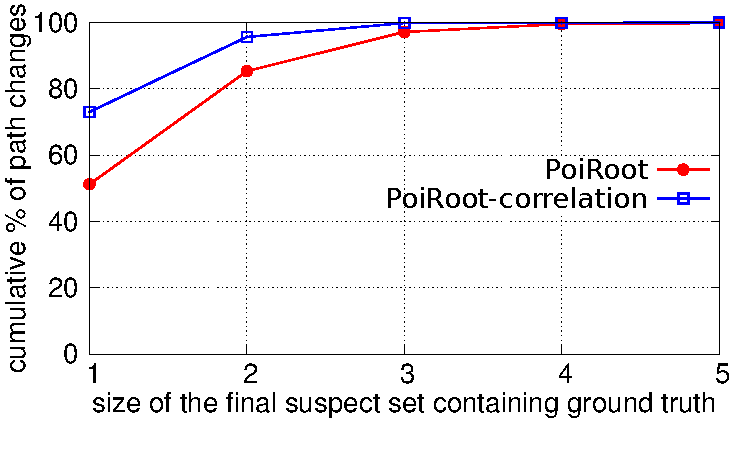
\includegraphics[width=\columnwidth]{figs/main.pdf} 
\vspace{-2em}
\caption{CDFs of the size of the final suspect set. \ouralgo, combined with an optimization that correlates the results across sources, results in a small suspect set on average as well as high accuracy.} 
\label{fig:main} 
\vspace{1em}
\end{figure}

\nparagraph{Comparison with \feldmann.}
We now compare our results with those from using \feldmann, which is based on the approach proposed by 
Feldmann et al.~\cite{feldman}.

%  We include two variations of the \feldmann algorithm:  The standard
%  version correlates path changes across vantage points (labeled
%  ``\feldmann-standard'', see \S\ref{sec:challenges}) and a slightly
%  modified version that considers each path change individually without
%  correlation (labeled `` \feldmann-individualPath''). 

The standard  \feldmann algorithm (see \S\ref{sec:challenges}) builds a suspect set that
contains the root cause for only 61.7\% of the path changes, but with an
average suspect set size smaller than that of our algorithm.  This suggests 
an inclusion policy that is too conservative and an elimination
policy that is too aggressive.  We now detail the reasons behind  
these issues.

A key reason for inaccuracy is that the standard \feldmann algorithm may
output an empty set when an induced path change is observed.  For
example, when AS $x$ causes an induced path change at another AS $y$,
$x$ may be identified as the root cause when considering paths from $x$,
but it does not appear on the new or old paths used by AS~$y$.  Because
the suspect sets from $x$ and $y$ may not overlap, the intersection may
produce an empty set. The impact of this limitation is significant: in
our experiments, 38.3\% of the path changes were due to an event that
generated an induced change. 

The existence of even a small number of induced path changes can
significantly decrease  \feldmann's accuracy.  In fact, a
larger set of available vantage points leads to a higher probability
that at least one induced change will be observed for a network event.
Out of the 292 RouteViews peers and PlanetLab nodes used in our system,
15.8\% observed at least one induced path change over the course of the
experiment. 

\begin{comment}
For example, assuming that observed path changes are independent, if the probability of an induced change at a randomly sampled vantage point is 0.05, 
for 20 of these vantage points, the probability of observing at least
one induced path change is $1-20^{0.95} \approx 0.64$. \fig~\ref{fig:induced-vp-cdf} is a histogram showing the percentage 
of the total number of vantage points in our system that observe at least X induced changes for a certain
value of X. As can be seen, more than 15\% of the vantage points experience at least one induced
change during the course of the experiment. 
\end{comment}

One way to address the induced path change problem is to modify the standard  \feldmann algorithm 
so that every path change is treated on an individual basis instead of
grouping all changes for an event (\feldmann-individualPath). This approach
avoids taking the intersection of the individual candidate sets. It still fails to deal with an induced change due to the  
assumption that the root cause lies on either the old or new path. However, it improves results for non-induced changes, 
increasing accuracy to 91.1\%. This comes at the cost of precision: the elimination
policy is less aggressive without correlation, so the median and mean suspect set size for correct identification is larger (2 and 2.7, respectively). 
This highlights a key limitation of \feldmann: the algorithm is either precise but not accurate; or in this case, 
accurate but not precise.  


%Feldmann et al. advocate, in addiction to their standard methodology, the 'better path' heuristic.
%This says that the root cause must lie on the more preferred or "better" of the old and new paths when compared head-to-head. This is because if the old path was better, the AS would only switch over to the 
%new path if something changed on the old path no matter the status of the new path. Similarly the root cause could not have been on the old path if the new path was better since the AS would not have been
%using the old path in the first place. Ignoring local preference, the 'better' path is taken to be the shorter
%path of the two. But since longer AS paths are quite often the more preferred paths due to policy considerations in practice, this heuristic performs poorly, yielding
%an accuracy of only 23.4\%. Another heuristic is correlation across prefixes. This is predicated on the observation that BGP updates to multiple prefixes are often correlated~\cite{feldman}. Since we perform different poisonings for different prefixes for our controlled announcements, this approach is not applicable here.

\nparagraph{Robustness to Missing Information.}
We now address the question of whether \ouralgo is robust to 
missing path information. Note 
that \ouralgo always includes the root cause in our suspect set unless a 
new path from a monitored AS $a$ uses an AS $b$ that never appeared in 
previous measurements. This case never occurred in our experiments. 
Thus we quantify the robustness of our approach by evaluating the precision of 
\ouralgo when previously available paths are removed from the dataset.

In particular, consider AS $x$ in our suspect set first discovered on the old path 
originating from AS $v$, hence $O(x)$ is known. Now our system measures 
$N(x)$. To determine how \ouralgo would 
perform with missing information, we set $N(x)=\mathit{missing}$ with probability $p$.
Similarly if $x$ were originally discovered on the new path from $v$, \ie 
$N(x)$ is known, we set $O(x)=\mathit{missing}$ with probability $p$.
Increasing $p$ causes \ouralgo to use the \textbf{MissingPath}
heuristic (from \S\ref{subsec:uncertainty}) more frequently; this in turn can increase 
the suspect set size. 

In \fig~\ref{fig:p-cdf} we plot the average suspect set sizes (and standard deviations) as 
we vary $p$. For each value of 
$p, 0 \leq p < 1$ we run the algorithm ten times on each path change and take the average 
suspect size. The final average for $p$ is taken over all these averages. We note that
the mean suspect set size increases slowly as $p$ is increased.
In fact the mean suspect size is less than 2 for a missing probability as large as 0.7. 

\ouralgo is robust to missing measurements because 
paths from multiple vantage points tend to overlap as they converge
toward the destination prefix. A single path measurement can remove
multiple ASes from the suspect set, even ASes added to the suspect set
due to missing measurements. For example, if \ouralgo observes a
\localC{} or a \neighborC{} at an AS $x$ (\S\ref{subsec:rules}), \ie $O(x) \neq N(x)$, all ASes upstream from $x$ are removed
since they cannot be the root cause. 

\begin{figure}[tbp]
\centering
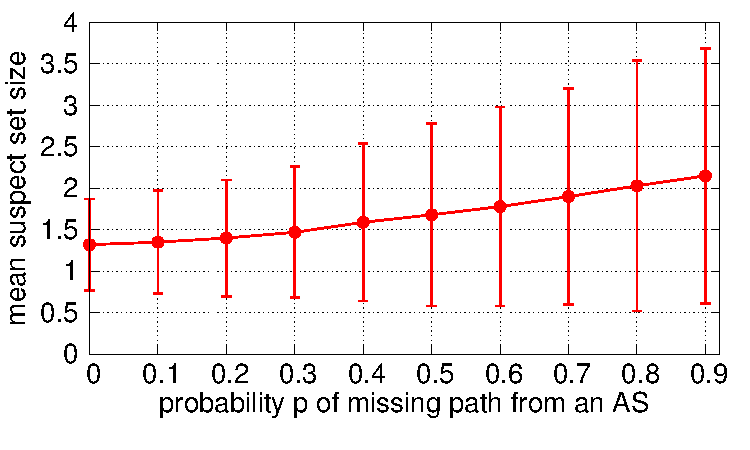
\includegraphics[width=\columnwidth]{figs/p-cdf.pdf} 
\vspace{-2em}
\caption{Mean suspect set size (and standard deviation) as we vary 
the probability of a missing path from an AS. \ouralgo is reasonably 
robust to missing path information: on average the suspect set size is 
only 2 when 70\% of paths are missing. }  
\label{fig:p-cdf} 
\vspace{.5em}
\end{figure}

\nparagraph{Prevalence of Induced Path Changes.}
One of the key strengths of \ouralgo is its success in dealing with
induced path changes. We showed earlier that even a small 
number of induced changes can significantly decrease the effectiveness
of previous approaches, such as \feldmann. Now using a combination
of our measurement data and the UCLA Internet graph~\cite{ucla-topology}, 
we argue that a larger set of vantage points would lead to significantly 
more observations of induced changes than in our controlled setting. 

To simulate the scenario where we have more vantage points, and thus
more paths, available to \ouralgo, we extend the empirically derived AS
topology used in the previous section. Specifically, for each AS $x$ in
our measured paths, we find its set of upstream neighbors from the UCLA
Internet graph. We use the corresponding annotated business
relationships to determine whether these neighbors are upstream. Then,
for each upstream neighbor $u$, we calculate the shortest valley-free
path from the neighbor toward a TP prefix. AS $u$ will use this path
only if it is shorter than the path exported by $x$.  We use path
changes from our poisonings to determine which ASes $x$ choose a longer
path over a short one. These ASes may cause an induced change at an
upstream AS $u$ if a failure occurs on $x$'s old path and $x$ selects a
new shorter path, \ie $N(x) < O(x)$. This is identical to the example in
\fig~\ref{fig:induced1}, where $y$ chooses a longer path and induces
changes at $v$. 

We find 302 cases where AS $x$ prefers a longer BGP path.
This leads to a total of 7555 induced path changes caused by just 55 simulated link failures.
Hence with a larger set of paths being monitored, the number of induced path changes increases. 
Therefore an approach that does not account 
for induced changes is more likely to be inaccurate as the number of vantage points increases.

We also run \ouralgo on this set of simulated induced path changes. 
\ouralgo continues to always include the root cause in its suspect set; 
the suspect set contains only the failed AS.
We also model missing paths with the parameter $p$ similar to \fig~\ref{fig:p-cdf}. The results 
are similar to \fig~\ref{fig:p-cdf}. For example, $p = 0.7$ results in a mean suspect size 
of 1.65.

\begin{comment}

\nparagraph{Varying the number of vantage points.}  A key question is
whether our algorithm will be effective even when path information is
missing.  We quantify this evaluating the precision of our algorithm
when data from only a subset of the vantage points are available.
\fig~\ref{fig:vp-cdf} shows that, indeed, our algorithm is effective in
face of missing path information.  We begin with paths from a total of
112 RouteViews peers monitors and 180 PlanetLab nodes.  For each path
change and for each fraction of vantage point availability (x-axis), we
select five random samples of vantage points.  We then run the algorithm
for each random sample of vantage points and the final suspect set size
is averaged over the five samples.  The error bars show the average and
standard deviation of the suspect set sizes\ic{I think median and
quartiles is more representative as the distribution is skewed toward
large suspect sets}.  The CDF shows a diminishing returns pattern as the
number of vantage points used is increased, with no significant
difference when we use more than 60\% of vantage points.  Note that the
accuracy, \ie the root cause lying in the final suspect set, is always
100\% since our \textbf{MissingPath} heuristic is conservative: it may
overestimate the size of the suspect set but never excludes the root
cause from it.\ic{Jelena: how many VPs would we need in the general
case?}\ic{i think it's easy to change the code (Umar should confirm) to
compute the fraction of ASes with missing path information and show it
in the y2axis.  this way we tie vp availability with measurement
availability.  even though we won't be able to make strong claims about
robustness to missing data in general (because we don't control data
availability directly), we can at least say that the suspect set size
does not explode when data availability decreases.  i also think the
question of how many VPs we would need in the general case is pretty
tough to answer; it seems to depend on the topology and VP location.}


The reason for this result is that many of our paths have shared segments, so portions 
of a path monitored by one VP will appear in at least one other path. 
In total 303 unique ASes appear on these paths; \fig~\ref{fig:asCommon-cdf} is the CDF of ASes in terms of the number of times each AS appears 
on a path from from our set of vantage points. 
\begin{figure}[tbp] 
\centering
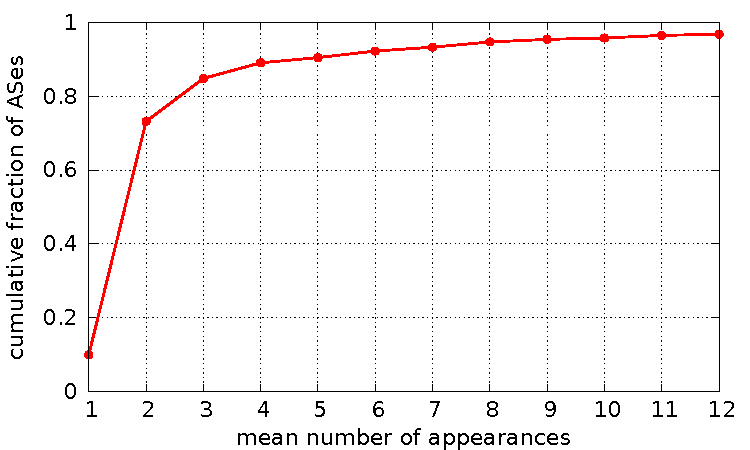
\includegraphics[width=\columnwidth]{figs/asCommon-cdf.pdf} 
\caption{} 
\label{fig:asCommon-cdf} 
\end{figure}
For this we announced an unpoisoned prefix from
the UWisc TP node and averaged the counts over 10 path snapshots collected every 90 minutes.
We exclude UWisc's ASN since it appears in every path. The figure shows that more than 80\% of the ASes
appear on more than one path, with more than 25\% of the ASes appearing on three or more paths.
\end{comment}

\nparagraph{Candidate and Monitored Set Bounds.} We now quantify the
scalability gains obtained with our bound on the candidate set.  We
compute the sizes of the general and bounded candidate sets
$\mathcal{C}(v)$ and $\mathcal{B}(v)$ for all path changes in our
poisoning experiments and also the sizes of the general and bounded
monitored sets $M(v)$ and $T(v)$.  We use exhaustive poisoning
experiments---we need topology information as complete as possible to
compute the general candidate and monitored sets $\mathcal{C}(v)$ and $M(v)$

The further an AS is from the origin AS (\ie our TP providers), the
longer its paths and the larger its candidate and monitored sets.  We
compute candidate and monitored sets for the ASes where we have vantage
points because they are the furthest from the origin AS in our dataset.
We also note that the bounded candidate and monitored sets
$\mathcal{B}(v)$ and $T(v)$ depend on $v$'s old path $O(v)$; in
particular, the size of $T(v)$ depends heavily on the preference rank of
its old path.  The general candidate and monitored sets $\mathcal{C}(v)$
and $M(v)$ are independent of $O(v)$.

\begin{figure}
\begin{center}
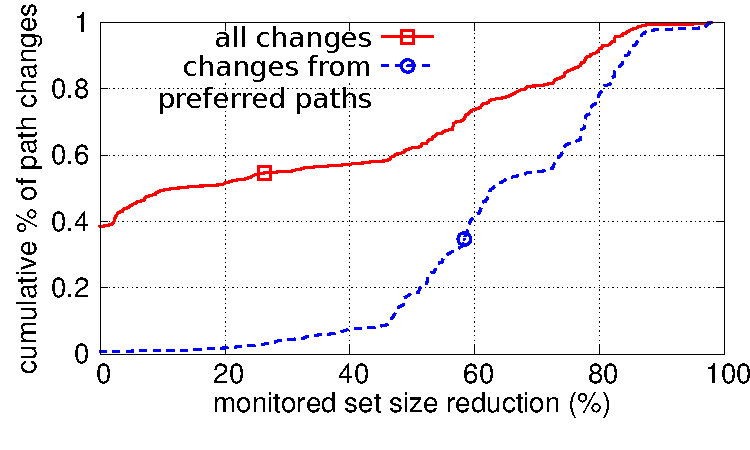
\includegraphics[width=1.0\columnwidth]{figs/scalability_monset_gains.pdf}
\vspace{-2em}
\caption{Our bound on the candidate set size allows us to reduce the
number of ASes we have to monitor to perform root cause analysis.}
\label{fig:setsizes}
\end{center}
\end{figure}

The solid line in \fig~\ref{fig:setsizes} shows the distribution of the
reduction in monitored set size (\ie $|M(v) - T(v)|\div|M(v)|$) across
all path changes in the data set.  Overall, we reduce the monitored set
size by more than 50\% for 38\% of path changes.  The average size of
the general and bounded monitored sets are $E[M(v)] = 38.9$ and $E[T(v)]
= 27.0$, and the average reduction in size is 31\%.  The bounded
monitored set is identical to the general monitored set for 38\% of the
path changes (where the solid line intersects the $y$-axis).  This
happens whenever an AS is using its least preferred path, as we have
to monitor all other paths that are more preferred.  Even if an AS is
not using its least preferred path, the set of ASes to monitor
quickly converges to the general monitored set as the number of more
preferred paths we need to monitor increases.  

The dashed line in \fig~\ref{fig:setsizes} shows the reduction in
monitored set size across the subset of path changes when an AS $v$
changes from its most preferred path to an arbitrarily less preferable
path.  Because we only need to monitor a few less preferred paths when
$v$ is using its most preferred path, the reduction in monitored set
size is significantly higher.  The average reduction in this case is
65\%.  

The reduction in candidate set sizes (\ie
$|\mathcal{C}(v)-\mathcal{B}(v)|\div|\mathcal{C}(v)|$) is much smaller
(not shown), as induced path changes are rare in practice and we do not
observe any 3-level induced path changes.

\nparagraph{Detection Speed.} 
To allow providers and operators to debug problems caused by 
path changes in real time, we would like \ouralgo to provide 
root cause analysis as changes occur. Our current system refreshes 
paths from traceroutes every 10 minutes and from BGP feeds 
every 15 minutes. The algorithm for generating the suspect set 
takes seconds to run, so our system currently can provide results 
at the same rate that paths are refreshed (\ie 15 minutes or less). 
We note that we can 
further reduce detection time by monitoring real-time BGP feeds 
(\eg via BGPMon~\cite{bgpmon-pub}) and triggering path measurements 
on demand in response to issues such as performance problems. 

\subsection{In the Wild Path Changes}
\label{sec:eval-real}

Having shown that our approach is accurate and precise
for path changes obtained by controlled BGP poisonings and simulations,
we now demonstrate its effectiveness for path changes seen ``in the
wild.'' 
In particular, we focus on path changes that significantly worsen end-to-end latency, 
as they are most likely to warrant further debugging from service providers and 
operators that optimize for performance.

\subsubsection{Methodology}
We identify path changes as follows. We issued traceroutes between all PlanetLab sites every ten minutes for
a period of three days starting November 1st, 2012, and perform IP-to-AS
translation to convert traceroutes to AS-level paths.  
We extract from this dataset AS-path changes that last for at least an hour. 
In addition we require that the path before the change is stable for at least
30 minutes to allow for convergence.  

Since network operators will be most interested in further investigating those 
path changes that degrade performance significantly, we use 
the relative change in RTT as our performance metric and consider only those
path changes that experience an increase in RTT larger than 10ms and whose
relative increase in RTT is greater than 25\%. Each RTT value is averaged over
at least three samples. This gives us a set of 643 path changes for the three day
period. 

\subsubsection{Results}

\fig~\ref{fig:real-world-rc} shows the distribution of the size of the
suspect set built by \ouralgo with the \textbf{Correlation} 
heuristic for the
path changes identified above, as well as the 
corresponding distribution from controlled experiments \S\ref{sec:poisonings}. The
results are similar: the suspect set size is one AS for more than 64\%, and to two ASes 
for more than 83\% of the path changes. We find that 96\% of the suspect sets with more than
one AS include a sequence of consecutive ASes (\ie ASes are adjacent).

\begin{figure}[t]
\centering
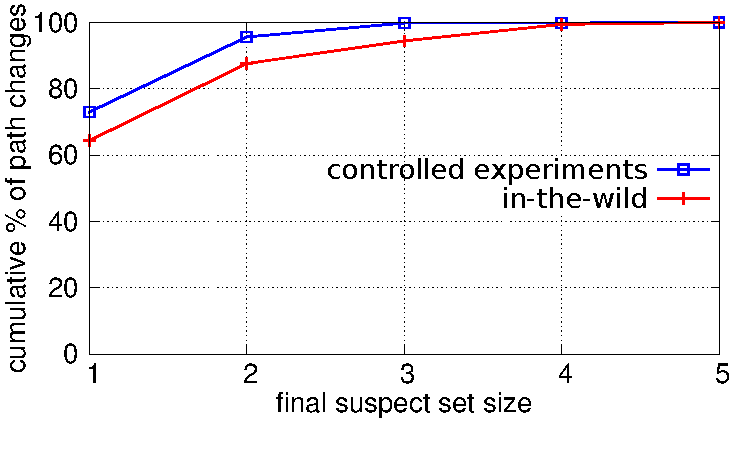
\includegraphics[width=\columnwidth]{figs/real-world.pdf}
\vspace{-2em}
%
\caption{Distribution of suspect set sizes built by \ouralgo running on
	path changes observed ``in the wild''. The
corresponding CDF from \S\ref{sec:poisonings} is shown
as well. Our algorithm identifies the root cause as being one or two ASes for
more than 84\% of the cases.}
%
\label{fig:real-world-rc}
\vspace{1em}
\end{figure}
